\documentclass[11pt]{article}
\usepackage{geometry}                % See geometry.pdf to learn the layout options. There are lots.
\geometry{letterpaper}                   % ... or a4paper or a5paper or ... 
%\geometry{landscape}                % Activate for for rotated page geometry
%\usepackage[parfill]{parskip}    % Activate to begin paragraphs with an empty line rather than an indent
\usepackage[pdftex]{graphicx}
\usepackage{amssymb}
\usepackage{epstopdf}

\usepackage[T1]{fontenc}
\usepackage[scaled=0.8]{beramono}

%\DeclareGraphicsRule{.tif}{png}{.png}{`convert #1 `dirname #1`/`basename #1 .tif`.png}
\usepackage{listings} 

\lstset{%
  frame=none,
  xleftmargin=5pt,
  stepnumber=1,
  numbers=left,
  numbersep=5pt,
  numberstyle=\ttfamily\tiny,
  belowcaptionskip=\bigskipamount,
  captionpos=b,
  escapeinside={<|}{|>},
  tabsize=2,
  emphstyle={\bf},
  commentstyle=\it,
  stringstyle=\mdseries\ttfamily,
  showspaces=false,
  keywordstyle=\bfseries,
  morekeywords={in,do,print},
  columns=flexible,
  basicstyle=\sffamily,
  showstringspaces=false,
  morecomment=[l]\%,
}

\lstdefinelanguage{Enso}{%
  numbers=none,
  sensitive=true,
  morecomment=[l]{//},
  morecomment=[s]{/*}{*/},
  morestring=[b]",
  emphstyle={\bf},
  commentstyle=\it,
  stringstyle=\mdseries\ttfamily,
  showspaces=false,
  basicstyle=\ttfamily,
  morekeywords={schema,type},
  keywordstyle=\bfseries,
  columns=flexible,
  showstringspaces=false,
  morecomment=[l]\%,
}

\newcommand{\C}{\lstinline}

\lstset{language=Enso}

\newcommand{\Enso}{Ens\={o}}

\title{
\includegraphics[scale=0.25]{enso.jpg}\\  Managed Data:\\ Structure and Interpretation of Data in \Enso}
\author{William R. Cook and Tijs van der Storm}
%\date{}                                           % Activate to display a given date or no date

\begin{document}
\maketitle

\begin{abstract}
Managed Data allow programmers to define or modify the
fundamental data definition mechanisms in a programming language. 
The programmer can change the language used to describe data, implement
that language by writing or modifying interpreters, and
integrate the new data mechanisms with existing language
support for data access and manipulation. For example,
Managed Data allow programmers to override the field/method
access operator (the ``dot operator''). Managed Data allow
easy implementation of many aspects of data, including 
logging/subscription, access/change control, bidirectional 
relationships, invariants and validation.
A bootstrap process is used so that all data, including the
data used to implement Managed Data, is managed.
This paper describes the implementation of Managed Data
as the foundation of \Enso, a new programming system based on 
model interpretation.
\end{abstract}

\section{Introduction}

Mechanisms for organizing and managing data are a fundamental
aspect of any programming model. Most programing models provide
built-in mechanisms for organizing data. Well known approaches 
include \textit{data structure definitions} (as in Pascal, C, Haskell, ML),
\textit{object/class models} (as in Java, Smalltalk, Self), and \textit{predefined
data structures} (as in Lisp, Matlab).
Languages may also support type abstraction (as in ML, Ada), a combination of 
multiple approaches (e.g JavaScript, Scala), or other variations.
The key characteristic of all these approaches is that the
fundamental mechanisms for structuring and manipulating data are 
predefined.
Predefined data structuring mechanisms allow programmers to create
specific kinds of data, but they do not usually allow 
fundamental changes to the underlying data structuring and 
management mechanisms. 

Predefined data structuring mechanisms are insufficient to cleanly
implement many important and common requirements for data management,
including persistence, caching, serialization, transactions, change logging,
access control, automated traversals, 
multi-object invariants, and bi-directional relationships. 
The difficulty with all these requirements is that they are best 
implemented as pervasive features of the underlying data management
mechanism. It is possible to defined such features individually for
each particular kind of data in a program, but this typically leads to
large amounts of repeated code. To implement these kinds of crosscutting
concerns, developers often
resort to preprocessors, code generates, byte-code transformation, 
or modified runtimes or compilers. The resulting systems are typically ad-hoc,
fragile, poorly integrated, and difficult to maintain.

What is involved in making fundamental and potentially pervasive 
changes to the way data is managed in a programming model? There are
several ways to approach this question, but one concrete example is to
consider what it would mean to override the ``dot'' operator, which 
selects a field of a structure or object in many languages. One might also
consider a global override of the field assignment operator. Giving the
programmer control over the data manipulation mechanisms means defining
or modifying the behavior of all the data manipulation operations that
are often considered built-in primitives, including initialization, type tests, 
casting, pointer equality, and field access. In this view, the
data structuring mechanisms are an \textit{aspect} of an overall programming
system. 

Some programming systems support a degree of control over 
the data structuring mechanisms. Meta-classes in Smalltalk define how
classes are instantiated and compiled. 
The reflective features of Ruby, Python and Smalltalk 
can be used to trap and handle undefined methods and properties, 
which can be used to create proxies or implement virtual objects.
Scheme macros are often used to create data structuring mechanisms.
For example, the \lstinline{defstruct} macro defines mutable structures
with a functional interface. However... <summarize>. 
The Adaptive Object Model Architecture provides an architecture for
this approach, but does not discuss how it is bootstrapped or integrated
with existing languages.

This paper presents Managed Data, an approach to data definition
in which programmers have control over the data structuring 
mechanisms, either to define
new mechanisms or modify the system's built-in mechanisms. 
Managed Data has four main features: (1) high-level \textit{data models}
that specify the structure and behavior of data, 
(2) \textit{data model interpreters} that manage data instances, 
(3) \textit{programming language integration} so that managed instances
can be created and accessed just like normal data,
and (4) a \textit{bootstrapping} process
that allows all Managed Data, including data models, to be customized
and managed. Managed Data
places strong requirements on the host programming language, to 
support use-defined interpretation of data.

\section{Managed Data}

Managed Data allows a programmer to 
build libraries, or data managers, that implement the fundamental
data manipulation primitives in a programming language. 
Different approaches to Managed Data might be developed 
based on the choice of primitives to support. 

Figure~\ref{ddl} illustrates the difference between 
traditional built-in data structuring mechanisms and Managed Data.
In the traditional approach, the programming language includes a 
process and data sublanguages, which are both predefined.
With Managed Data, the data structuring mechanisms are defined
by the programmer by interpretation of data definitions.
Since a data definition model is also data, it requires a meta-definition
mechanism. This infinite regress is terminated by a boot-strap
data definition that is used to build the Managed Data system itself.

\begin{figure}
\begin{center}
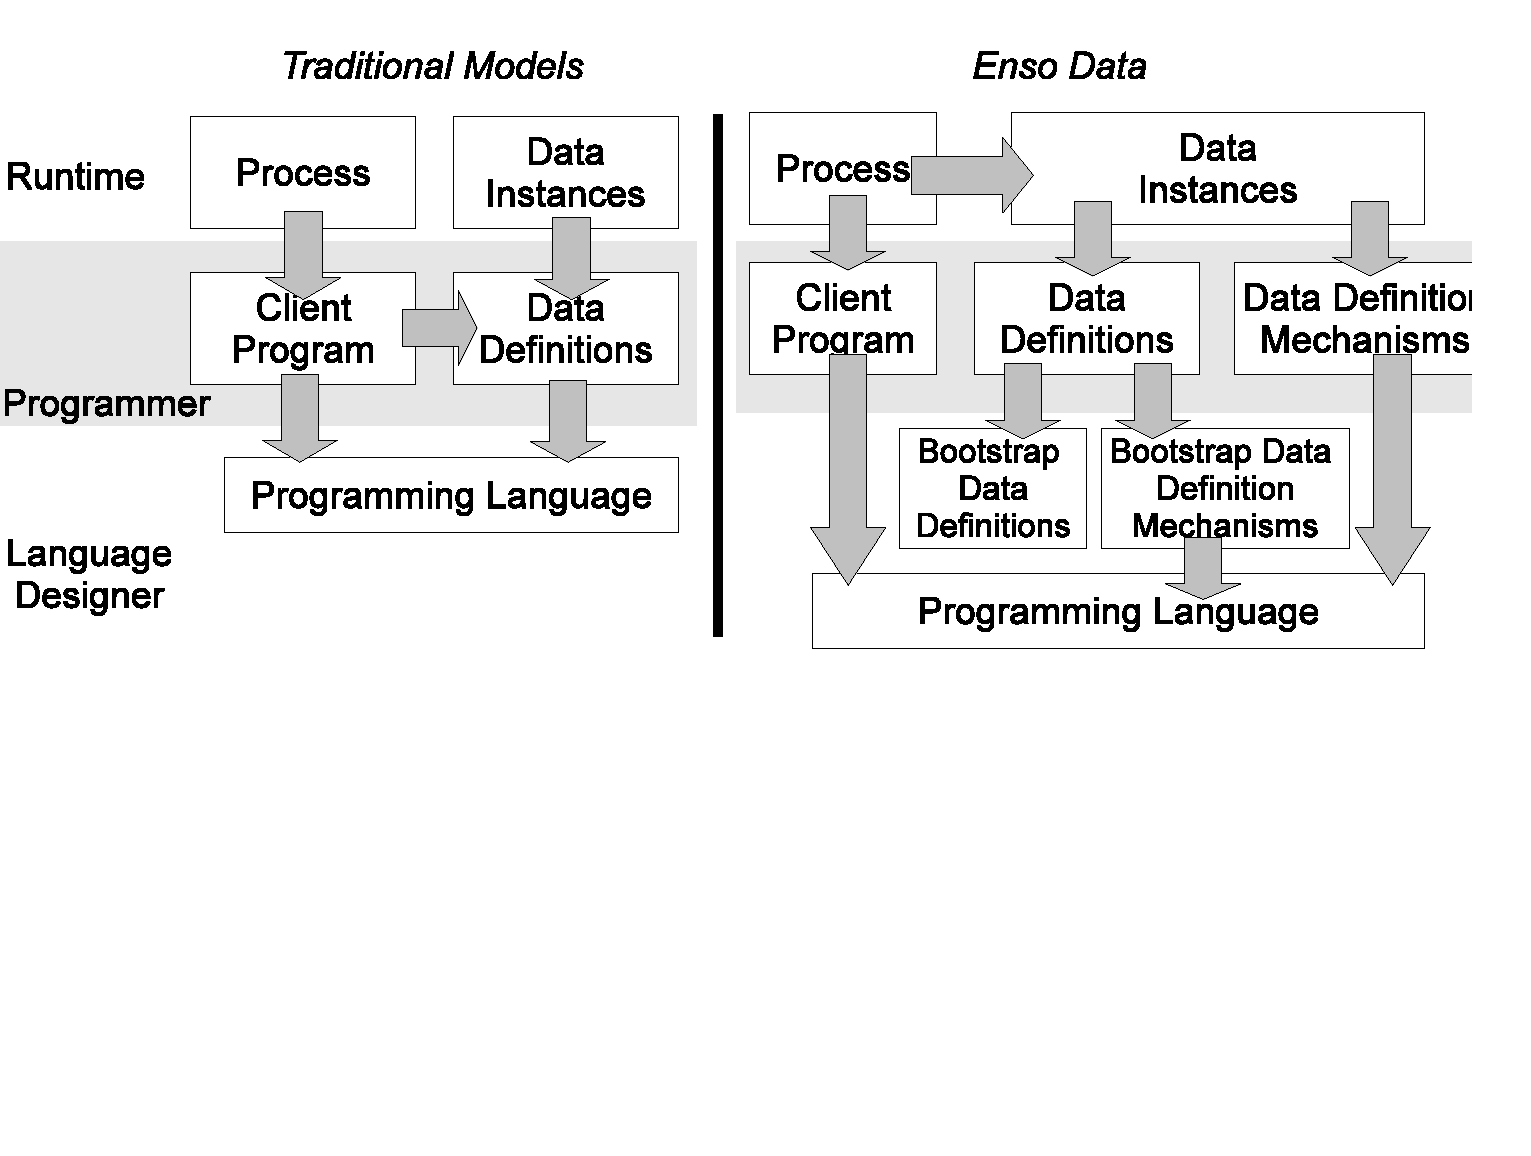
\includegraphics[scale=0.5]{DDL.pdf}
\caption{Traditional versus Managed data definitions}
\label{ddl}
\end{center}
\end{figure}

We develop an approach to Managed Data
based on primitives for \textit{construction},
\textit{component selection/update}, and \textit{case distinction}. We also define operations on
collections for \textit{indexed access}, \textit{insertion}
and \textit{deletion}. 
The concept of construction is common to all programming
languages and is usually implemented by defining an appropriate
function or procedure. 
Component selection \lstinline{o.f} corresponds to 
projecting a field of a labeled product, or record. 
Case distinction can be understood as analyzing the cases of a labeled sum,
or variant record. Object-oriented programming supports 
method dispatch as the preferred form of case distinction, 
although explicit type tests (\lstinline{instanceof}) may also be used. 
Indexed access \lstinline{a[k]} is used for arrays or maps,
where \lstinline{k} may be an integer or some other key.
Some languages use pattern matching to analyze and decompose data. 
However, pattern matching can be rewritten
using the more primitive operations of component selection and
case distinction.

One issue with implementing
the component selection operator is that its second argument
is a \textit{field name}. This requires that field names be
represented reflectively as values. In this paper we use Ruby
to implement Managed Data. In Ruby the form \lstinline{o.f}
can be implemented by defining a \lstinline{method_missing} method.
Figure~\ref{sdm} illustrates a simple data manager in Ruby.

\begin{figure}
\begin{lstlisting}
class SimpleDataManager
  def initialize(initial_values)
    @types = {}
    initial_values.each_pair { |key, value| @types[key] = value.class }
    @values = initial_values
  end
  def method_missing(name, *args)
    if name =~ /(.*)=/
      name = $1.to_sym
      raise "unknown field '#{name}'" if !@types.has_key?(name)
      raise "'#{name}' must be #{@types[name]}" if @types[name] != args[0].class
      @values[name] = args[0]
    else
      raise "unknown field '#{name}'" if !@types.has_key?(name)
      return @values[name]
    end
  end
end
\end{lstlisting}
\caption{A simple data manager in Ruby}
\label{sdm}
\end{figure}

There are at least two problems with this simple data manager.
One is that it only manages individual records, while we want to
manage collections of interrelated objects. A second problem
is that it is not reflexive, in that the input specification
to the data manager is not managed data. To address both these
issues, we need to define a richer data structuring mechanism
that is sufficiently powerful to be self-describing.

One more subtle issue is what organizational principle to use for
structuring data. 
Two obvious options are \textit{trees} or \textit{graphs}. Trees are
frequently used in functional languages and are appealing because
of their strong support for induction. Graphs can be 
created in any language with mutable
data structures, including object-oriented languages. 
However, this style of representation is essentially
node-oriented, as the graph emerges from the structure of connected
nodes rather than being described at the level of the graph itself.
Much of the work on model-driven development is done using graphs
and graph transformation. 
The relational model is also graph-based. 
Rows correspond to nodes and foreign keys are edges.
Graphs are explicit in the 
Entity-Relationship (ER) model \cite{FOO}, also known as Information
Models \cite{FOO}, and Class Diagrams in 
the Unified Modeling Language (UML) \cite{FOO}
The relational model also has a solid formal foundation, and 
subsumes trees as a special case.
But no general-purpose programming language, to our knowledge,
has used graphs as its primary data structure. While there may
be other ways to define Managed Data, we choose to investigate
the use of graphs to represent data in \Enso.

\subsection{Data Graphs}

Database = Table*
Table = Row*
Row = (Value, Value*)
Value = Number | String | Date




Structures in \Enso\ are a specialized kind of graph,
whose nodes are either primitive data or collections of observable
properties, whose values are either nodes or collections of nodes.
From a programming language viewpoint this may seem an odd 
choice for data representation. 
The key point is that structures in \Enso\ are 
viewed holistically as \textit{graphs}, not as individual values
or traditional sums-and-products data structures.

A structural description, or \textit{schema}, specifies some 
of the observable properties of structures. Schemas are used to
check the consistency structures. Some properties can be checked
while the structure is being created, but other can only be checked
once the structure is complete. \Enso\ allows modification of structures,
which is necessary to create cyclic graphs, but also allows 
valid structures to be sealed to prevent further changes.

\subsection{Schemas}

The following schema describes a collection of genealogy information:

\begin{verbatim}
schema GenealogySchema

  class Genealogy
    name: str
    members: Person*

  class Person
    name: str (key)
    birth: date
    female: bool
    father: Person?
    mother: Person?
\end{verbatim}

In a schema, a \textit{class} defines a kind of value, which is
followed by its properties or \textit{fields}. Each field has a name
and a type, where the type may be followed by \C|*| to indicate a 
many-valued field, or by \C|?| to indicate an optional value.
In this case, \C|Genealogy| has \C|members| which is a set of \C|Person|.
A \C|Person| has a \C|name| string, a \C|birth| date, and a \C|father| and \C|mother|,
which are optional \C|Person|s. The \C|father| and \C|mother| are optional
because every geneology is partial, so that not all fathers and mothers
can be included.

\subsection{Instances}

A particular collection of genealogy information, which conforms to the
above schema, might be written as follows:

\begin{verbatim}
Genealogy "Sam's Ancestors"
Person "Albert Snook"  11/1/89 male  +"Jane Snook" ^"Thomas Snook"
Person "Jane Snook"    3/17/48 female 
Person "Thomas Snook" 12/30/43 male 
\end{verbatim}

\subsection{Collections}
\subsubsection{Bags and Sets}
\subsubsection{Keys}

\subsection{Inverses}

\subsection{Computed Attributes}

\subsection{Invariants}

\subsection{Constraints}

\subsection{Modularity}

\section{Interpretation}

Model -> Behavior

\subsection{Factories}

Structure are created by \textit{factories}, which create
and manage the nodes in the structure. The factory also
ensures that structures are distinct: a factory identifies the 
collection of nodes that belong to a graph, and any given node 
can only be connected to other nodes in the same graph, which were
created by the same factory.

In \Enso\ most properties of a structure are
checked when the structure is being created. In other words, 
the \textit{factory} that creates the structure is parameterized by a
schema, which the factory uses to check the legality of operations
on the objects it creates.

\subsection{Instance Modification}

change tracking

Managed Data supports controlled imperative effects. Objects are
mutable during construction or modification, while the data may be in an
inconstent state, but before it can be used it must be validated
and locked from further changes. This is similar to a transaction.


\subsection{Differences}


\subsection{Instantiation}



\section{Programming Language Integration}

The programming model is based on cyclic graphs.
Graphs are kept distinct from each other. That is,
each graph is considered a self-contained
artifact, without links or pointers to other graphs.

A natural way to create such graphs is with 
imperative effects.

This potentially requires more copying of data
than would be the case in tree-based representations.

To modify graphs, place-holder objects are useful,
as is the ability to ``become'' another object.

\subsection{Simple reflection}

Fields can be created dynamically and accessed with
``.'' notation or reflective access.

\begin{verbatim}
o.foo   == o.get("foo")
\end{verbatim}

Assignment to fields can be overriden
\begin{verbatim}
   o.bar = 3   ==> o.set("bar", 3)
\end{verbatim}

\subsection{Dynamic Objects}

\section{Bootstrapping}


\subsection{QuadModel}


\begin{figure}[htbp]
\begin{center}
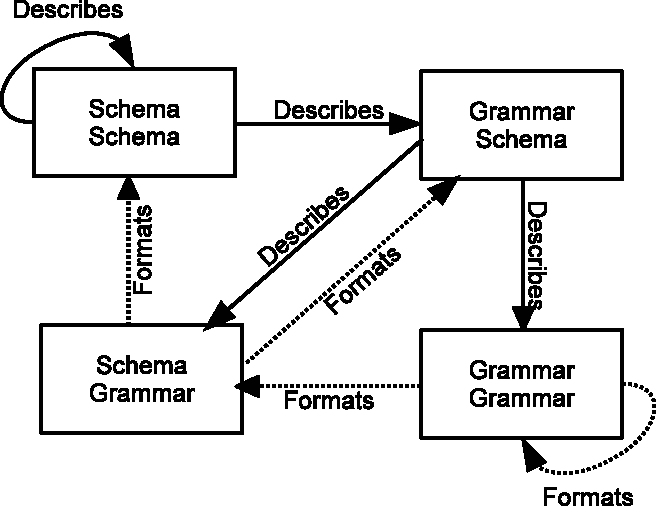
\includegraphics[scale=0.7]{QuadModel.pdf}
\caption{The four core schema and grammar models}
\label{default}
\end{center}
\end{figure}



\section{Related Work}
\label{relatedwork}

Managed Data is based on traditional 
entity-relationship (ER) models \cite{FOO},
which are also known as information models. 
ER models were the basis for class diagrams in UML.

In contrast to
object-oriented programming, \Enso\ is focused on holistic
object graphs, rather than individual objects. \Enso\ 
does allow data to include some behavior, for example constraints
and computed fields, but \Enso\ does not associated methods
with data objects.

The rendering transformation is similar to Smaragdakis's notion of
Morphing \cite{Morphing} (or is it SafeGen?). 
However, \Enso\ generalizes the transformation
so that any kind of structure can be morphed into any other
kind of structure. On the other hand, \Enso\ is not statically
typed.

\subsection{Other Related Work}

Look up work on "instant-generics"

Dave Clarke, Michiel Helvensteijn, and Ina Schaefer. 2010. Abstract delta modeling. In Proceedings of the ninth international conference on Generative programming and component engineering (GPCE '10). ACM, New York, NY, USA, 13-22. DOI=10.1145/1868294.1868298 http://doi.acm.org/10.1145/1868294.1868298 

\subsection{FOSD}

- Forests are the key data structure in a formal model of FOSD [1]. The goal is similar to yours: be language-independent and represent object collaborations.

- Recently, forests have been extended to graphs to encode more semantics and to support more automatic reasoning activities [2].

- Operations on forests (e.g., composition or conflict detection) are defined generically and can be plugged in on demand [3].

- The entire FOSD model is language-independent and has been used with many different artifact types (e.g., Java, C, Haskell, Alloy programs) [3].

- FOSD tools (the internal parsers and reasoning tools) are generated based on annotated grammars, whose annotations supply semantic information [3].

- The entire forest/grammar/annotation-based model has been enriched by adding behavior to features [4]. 

[1] Sven Apel, Christian Lengauer, Bernhard M�ller, and Christian K�stner. An Algebraic Foundation for Automatic Feature-Based Program Synthesis. Science of Computer Programming (SCP), 75(11):1022�1047, November 2010.

[2] Sven Apel, Wolfgang Scholz, Christian Lengauer, and Christian K�stner. Language-Independent Reference Checking in Software Product Lines. In Proceedings of the International Workshop on Feature-Oriented Software Development (FOSD), pages 65�71. ACM Press, October 2010.

[3] Sven Apel, Christian K�stner, and Christian Lengauer. FeatureHouse: Language-Independent, Automated Software Composition. In Proceedings of the ACM/IEEE International Conference on Software Engineering (ICSE), pages 221�231. IEEE Computer Society, May 2009.

[4] P. H�fner, R. Khedri, B. M�ller. Supplementing Product Families with Behaviour. International Journal of Software and Informatics, 2011. To appear. 

Dave Clarke, Michiel Helvensteijn, Ina Schaefer. Abstract delta modeling. GPCE'10



\end{document}  



\begin{verbatim}
schema Geometry

class Shape

class Point < Shape
  x: int
  y: int

class Rectangle < Shape
  upper_left: Point
  lower_right: Point

class Circle < Shape
  center: Point
  radius: int

class Polygon < Shape
  points: Point*
  
class Composite < Shape
  items: Shape*
\end{verbatim}

It says that the class \C|Point| has fields \C|x| and \C|y|.
--------
This example converts schemas into constructor grammars
\begin{verbatim}
grammar NAME:sym
   CLASSES:
     rule NAME:sym = 
        (SUBTYPES: { NAME:sym "|") "|" @"!SUBTYPES.empty?")?
         [NAME:sym] NAME:str "{" 
            FIELDS: { (NAME:str ":" (NAME:sym): (
                 "[" { TYPE.NAME:sym^ "," } "]"   @"MANY=true"
               | TYPE.NAME:sym^ ?                  @"OPTIONAL=true"
               | TYPE.NAME:sym^
               )) ";" }
             "}"
\end{verbatim}
